\chapter{統計学の基礎}
\label{chap_Statistics}

実験データの解析作業の目的のひとつは、何らかの物理量をそこから抽出し、その値が統計学的にどれだけ正しいかを評価することです。例えば電子の質量が約511~keVであることを私たちは知っていますが、その真の値がいくつかは誰も知りません\footnote{光速$c$のように299~792~458~$\mathrm{m}/\mathrm{s}$と正確に「定義」されている物理量も存在します。}。物理実験から統計学的な表現で言えるのは、電子質量は
\begin{equation}
  m_\mathrm{e} = 510.998\,946\,1\pm0.000\,003\,1\,\mathrm{keV}
\end{equation}
ということだけであり\cite{Patrignani:2016:Review-of-Particle-Physics}、これは510.998~946~1~keVがこれまでの実験でわかった最も良い電子質量の推定値であり、その誤差は0.000~003~1~keVである、もしくは言い方を変えると、約68\%の確率\footnote{より正確には約$68.27$\%であり、これは正規分布の$\pm1\sigma$の範囲に入る確率です。}で0.000~003~1~keVの範囲に収まっているという意味です。



\section{様々な確率分布}
\subsection{正規分布}
\subsection{ポアソン分布}

\lstinputlisting[language=c++,float=tb,caption=\texttt{Poisson.C},label=code_Poisson,numbers=left]{src/Poisson.C}

\begin{figure}
  \centering
  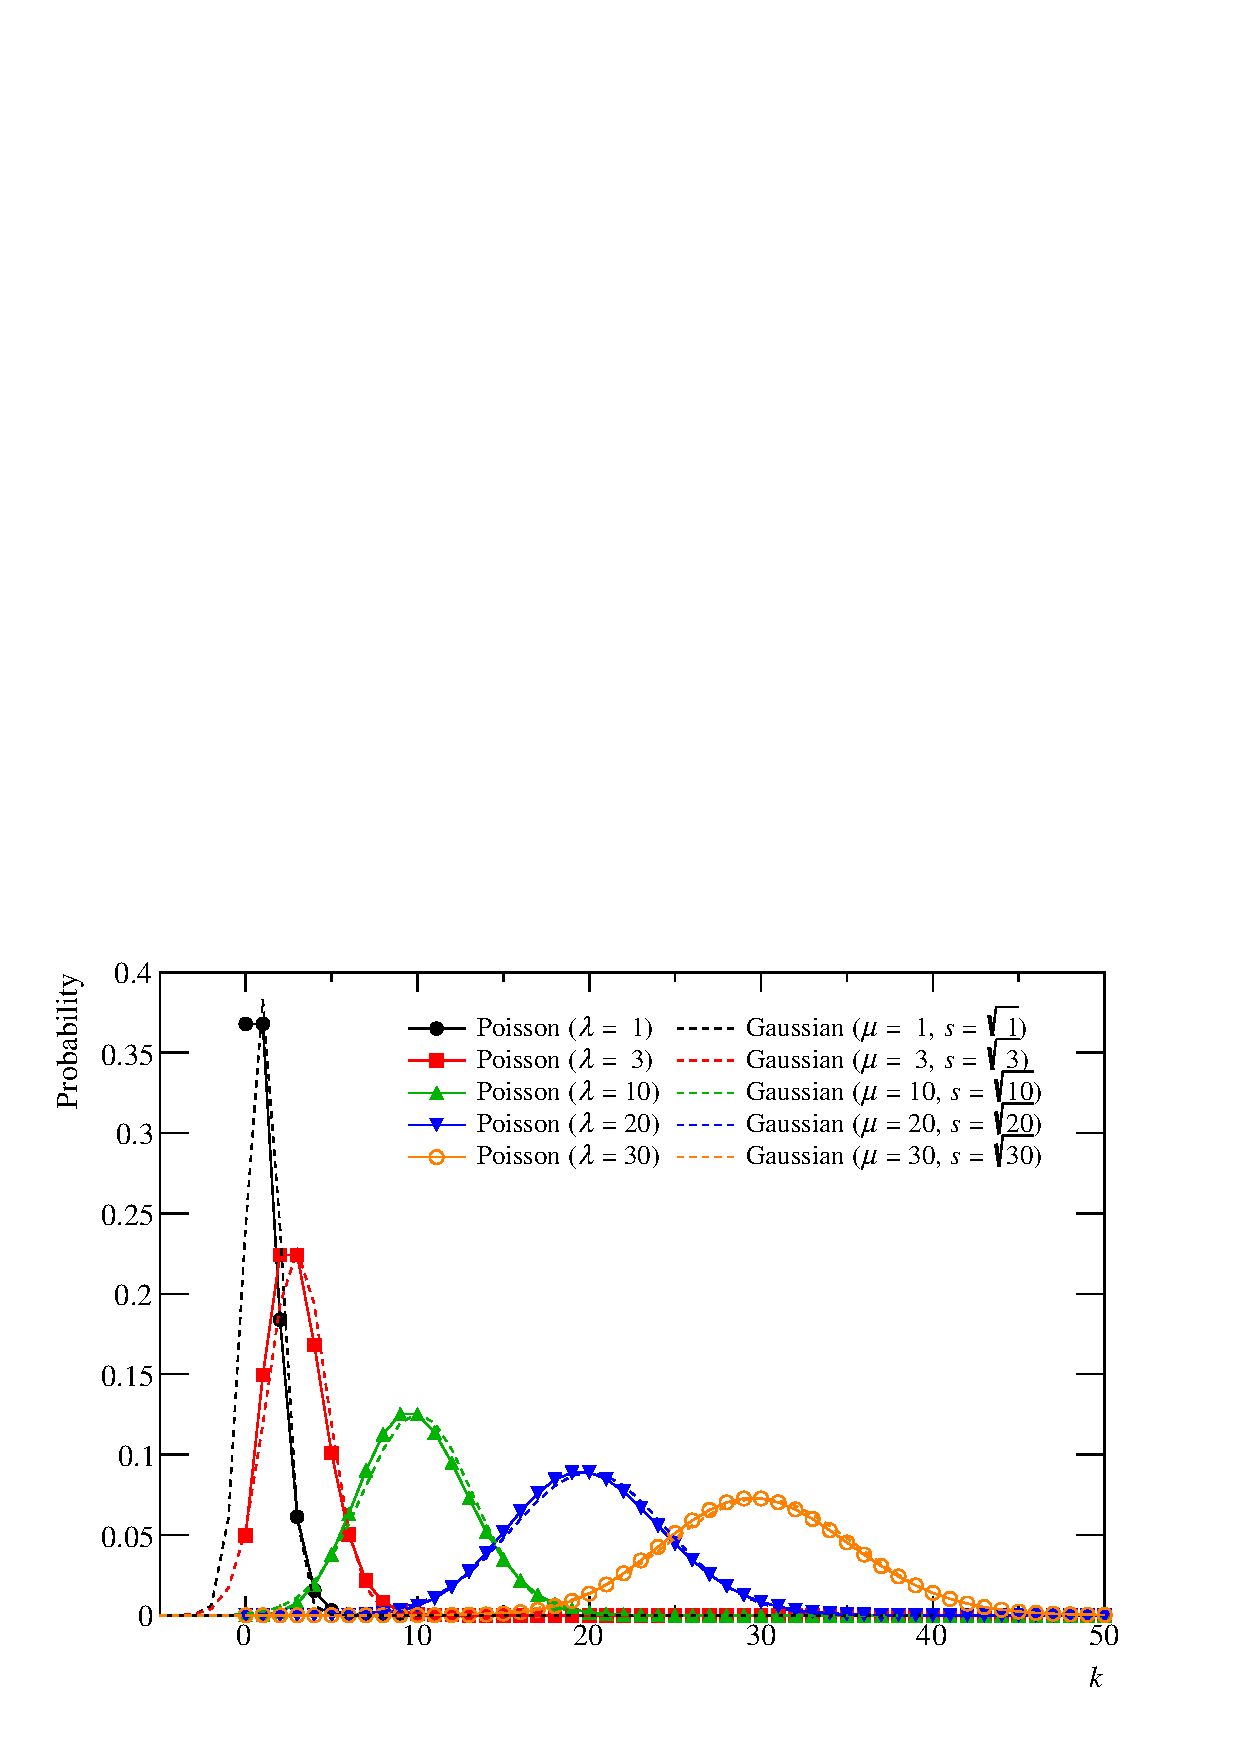
\includegraphics[width=12cm]{fig/Poisson.pdf}
  \caption{様々な平均値を持つポアソン分布と正規分布の比較}
  \label{fig_Poisson}
\end{figure}

\subsection{指数分布}
\subsection{二項分布}
\subsection{カイ二乗分布}

